\documentclass[journal]{IEEEtran}

%\usepackage[retainorgcmds]{IEEEtrantools}
%\usepackage{bibentry}
\usepackage{xcolor,soul,framed} %,caption

\colorlet{shadecolor}{yellow}
% \usepackage{color,soul}
\usepackage[pdftex]{graphicx}
\graphicspath{{../pdf/}{../jpeg/}}
\DeclareGraphicsExtensions{.pdf,.jpeg,.png}

\usepackage[cmex10]{amsmath}
%Mathabx do not work on ScribTex => Removed
%\usepackage{mathabx}
\usepackage{array}
\usepackage{mdwmath}
\usepackage{mdwtab}
\usepackage{eqparbox}
\usepackage{url}


% ----------------------------------------------

% Definitions of languages: ------------
\usepackage{listings}
\lstdefinestyle{cStyle}{
  basicstyle=\scriptsize,
  breakatwhitespace=false,
  breaklines=true,
  captionpos=b,
  keepspaces=true,
  numbersep=5pt,
  showspaces=false,
  gobble=4,
  tabsize=4,
  showstringspaces=false,
  showtabs=false,
}
\renewcommand*{\lstlistingname}{Code}

% ----------------------------------------------




% \hyphenation{op-tical net-works semi-conduc-tor}

%\bstctlcite{IEEE:BSTcontrol}


%=== TITLE & AUTHORS =========================================================
\begin{document}
\bstctlcite{IEEEexample:BSTcontrol}
    \title{Deep Q-Learning}
  \author{Carlos~Matheus~Barros~da~Silva,
  ~\IEEEmembership{Computer Engineering Bachelor Student of ITA}
  \\Prof. Marcos~Ricardo~Omena~de~Albuquerque~Máximo}

% The paper headers
\markboth{INSTITUTO TECNOLÓGICO DE AERONÁUTICA, July~2019
}{Deep Q-Learning}

% ============================================================================
\maketitle


% === ABSTRACT ===============================================================
% ============================================================================
\begin{abstract}

This paper evaluates a Deep Q-Learning technique applied to solve the \textit{Mountain Car} problem.

The technique have been implemented and passed by the test executing the \textit{Mountain Car} problem.
Both techniques have been implemented and passed by some tests. On the end It was avaliated the learning with a car that needs to follow a track.

It was observed that the implementation worked as expected. The \textit{Q-Learning} had a fast learning by the end being able to complete the challange in less than 50 traines.

% === KEYWORDS ===============================================================
% ============================================================================
\begin{IEEEkeywords}
    Q-Learning, Reinforcement Learning, Mountain Car
\end{IEEEkeywords}
\end{abstract}

\IEEEpeerreviewmaketitle

% ============================================================================
% ============================================================================
% ============================================================================


% === I. INTRODUCTION ========================================================
% ============================================================================
\section{Introduction}

\IEEEPARstart{R}{e}inforcement learning (RL) is an area of machine learning concerned with how software agents ought to take actions in an environment so as to maximize some notion of cumulative reward. Reinforcement learning is one of three basic machine learning paradigms, alongside supervised learning and unsupervised learning.

It differs from supervised learning in that labelled input/output pairs need not be presented, and sub-optimal actions need not be explicitly corrected. Instead the focus is finding a balance between exploration (of uncharted territory) and exploitation (of current knowledge).

The environment is typically formulated as a Markov decision process (MDP), as many reinforcement learning algorithms for this context utilize dynamic programming techniques. The main difference between the classical dynamic programming methods and reinforcement learning algorithms is that the latter do not assume knowledge of an exact mathematical model of the MDP and they target large MDPs where exact methods become infeasible.

Q-learning is a model-free reinforcement learning algorithm. The goal of Q-learning is to learn a policy, which tells an agent what action to take under what circumstances. It does not require a model (hence the connotation ``model-free'') of the environment, and it can handle problems with stochastic transitions and rewards, without requiring adaptations.

For any finite Markov decision process (FMDP), Q-learning finds a policy that is optimal in the sense that it maximizes the expected value of the total reward over any and all successive steps, starting from the current state. Q-learning can identify an optimal action-selection policy for any given FMDP, given infinite exploration time and a partly-random policy. ``Q'' names the function that returns the reward used to provide the reinforcement and can be said to stand for the ``qualit'' of an action taken in a given state.

% ============================================================================
\section{Deep Q-Learning Implementation}

The technique implementation can be seen on the file \textit{dqn\_agent} and on \textit{utils.py}. The essence of the implementation can be seen from the Code \ref{code:dqn} and to the Code \ref{code:reward}.

\lstinputlisting[
    language=python,
    caption={Code of the method \textit{make\_model}, that will crate the Neural Network},
    label={code:dqn},
    style=cStyle,
    firstline=42,
    lastline=86
]{./../code/dqn_agent.py}

\lstinputlisting[
    language=python,
    caption={Code of the method \textit{act} that will choose a $\epsilon$-greedy action.},
    label={code:act},
    style=cStyle,
    firstline=86,
    lastline=103
]{./../code/dqn_agent.py}

\lstinputlisting[
    language=python,
    caption={Code that implements the reward for a given state and next\_state},
    label={code:reward},
    style=cStyle
]{./../code/utils.py}

\section{Deep Q-Learning Analysis}

\subsection{Initial Training}

In order to train the model, it was used the \textit{dqn\_training}.

With this, it was obteined the graph represented on the Figure \ref{fig:train} that is the reward per training episode.

\begin{figure}
  \begin{center}
  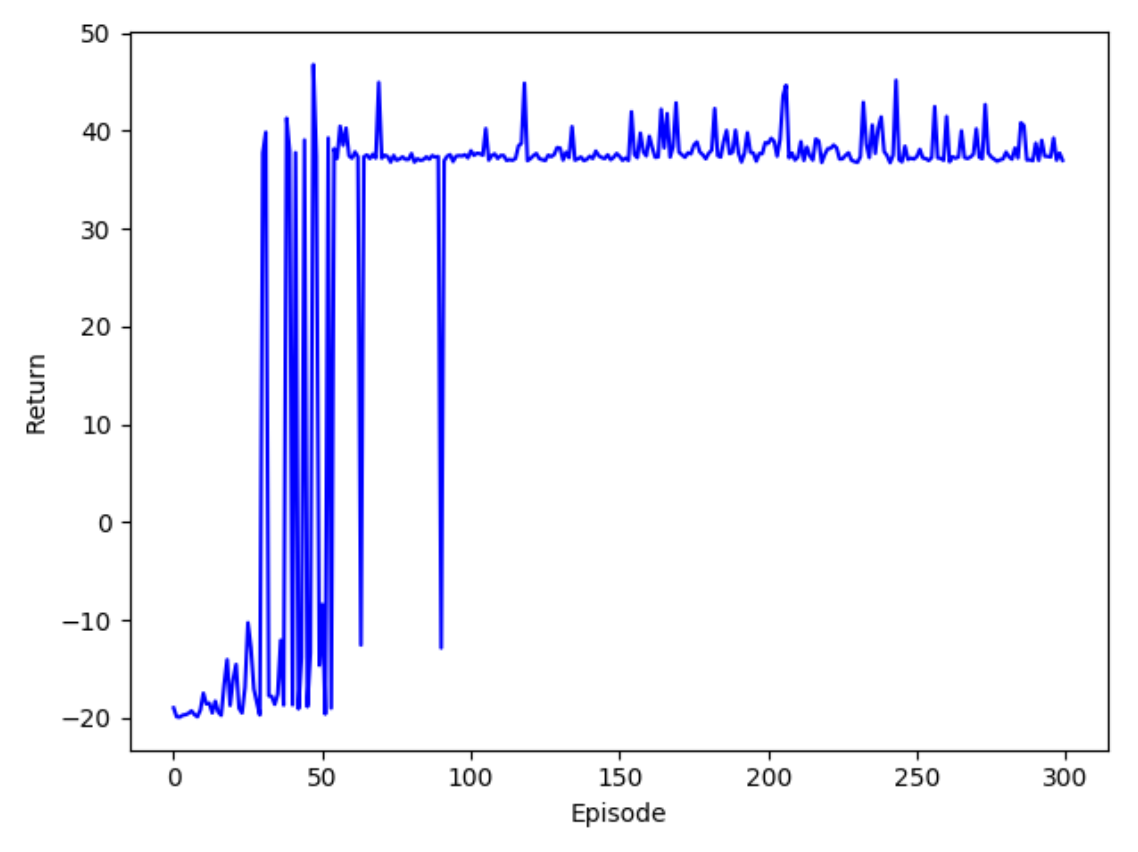
\includegraphics[width=2.8in]{./../code/output/first_train.png}
  \caption{Reward per training episode.}
  \label{fig:train}
  \end{center}
\end{figure}

As it is observed, the learning was fast, in way that after the 50th trainging the car was almost ways clibing the montain, and after the 100th it always climbed the mountain.

\subsection{Evaluating the Trained Model}

In order to evaluate the trained model it was used the script \textit{evaluate\_dqn.py}.

With it, was obtained the graphs represented on Figure \ref{fig:evaluate} and on Figure \ref{fig:policy}.

\begin{figure}
  \begin{center}
  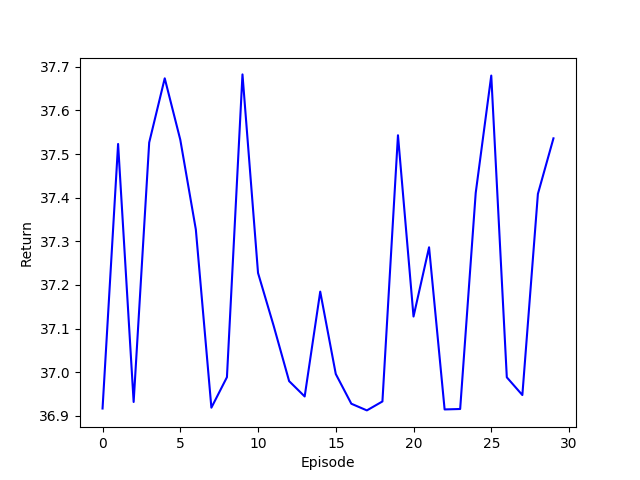
\includegraphics[width=2.8in]{./../code/output/dqn_evaluation.png}
  \caption{Reward per evaluation episode.}
  \label{fig:evaluate}
  \end{center}
\end{figure}

\begin{figure}
  \begin{center}
  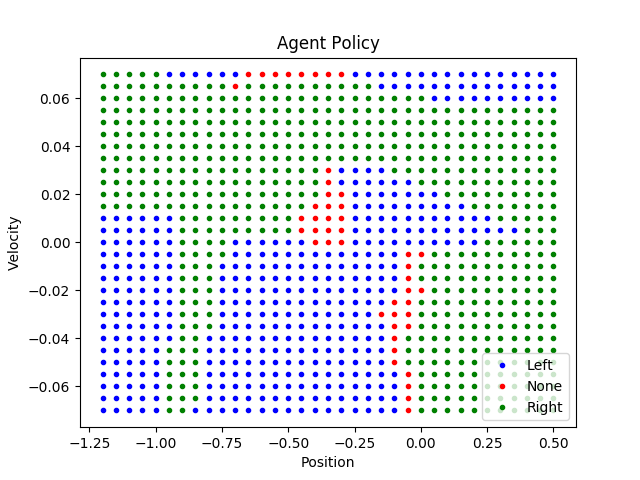
\includegraphics[width=2.8in]{./../code/output/agent_decision.png}
  \caption{Final Agent Policy.}
  \label{fig:policy}
  \end{center}
\end{figure}

It was observed that the convergency was good, the evaluation seen on Figure \ref{fig:evaluate} show that the returned reward was stable during the 30 tests.

With the Figure \ref{fig:policy} is clear the actions taken per region, it also has soft transitions with well determined actions regions, what makes sense to a well converged policy.

\section {Conclusion}

Is was clear, therefore, that the implementation worked as expected. The \textit{Deep Q-Learning} had a fast learning and good convergency, what garanteed a good solution to Montaion Car problem.

At the end of the learning the success rate was near 100\% at the training, having 100\% success rate at evaluation. Thus it is possible to conclude the algorithm solved the problem.

\vfill
\end{document}
